\section{Selected Article} % Seções são adicionadas para organizar sua apresentação em blocos discretos, todas as seções e subseções são automaticamente exibidas no índice como uma visão geral da apresentação, mas NÃO são exibidas como slides separados.

\begin{frame}{Selected Article}
\frametitle{Selected Article}
   \begin{figure}[h]
       \centering
       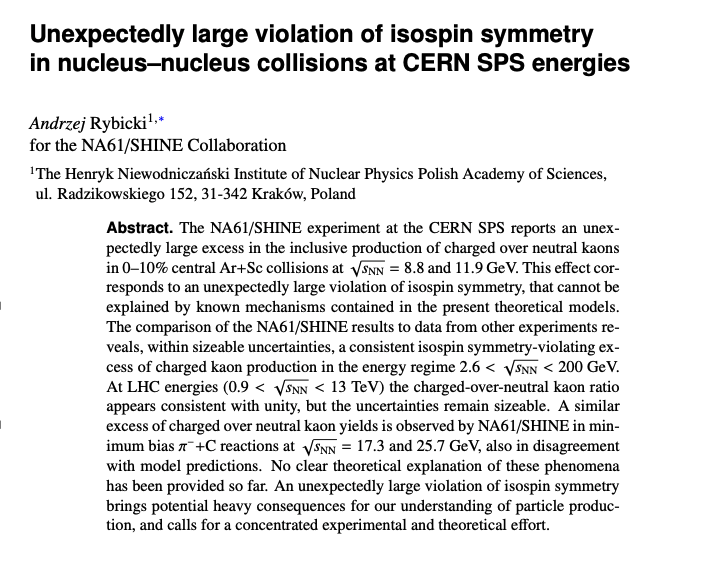
\includegraphics[width=0.65\textwidth,height=0.62\textheight,keepaspectratio]{img/selected_article.png}
       \caption{Isospin symmetry violation in nucleus--nucleus collisions.}
       \label{fig:selected_article}
   \end{figure}
\end{frame}

% \begin{frame}{Results}
% \frametitle{Results}
%    \begin{figure}[h]
%        \centering
%        \includegraphics[width=0.4\textwidth]{img/some_results.png}
%        \caption{Posterior contours, for two observables, as correlation strength increases.}
%        \label{fig:some_results}
%    \end{figure}
% \end{frame}


% \begin{frame}{References}
%     \nocite{*}
%     \printbibliography
% \end{frame}


